\section{Sơ lược Cấu trúc Backend Hiện hữu và Cơ chế Hoạt động Luồng Dữ liệu}
\label{sec:backend_operation}

\subsection{Sơ lược Cấu trúc Hệ thống Backend Hiện hữu của Nhà trường}
Hệ thống Backend của Nhà trường được tổ chức theo kiến trúc phân lớp hướng dịch vụ gồm 4 tầng:
\begin{enumerate}
    \item \textbf{Tầng Định tuyến \& Middleware (Routing \& Security Middleware):} Tiếp nhận request HTTPS từ Mobile Gateway, giải mã Shared Secret JWT (\texttt{session.ts}), kiểm tra tính hợp lệ của token và phân quyền RBAC (\texttt{authorize.ts}) dựa trên quyền hạn của cán bộ.
    \item \textbf{Tầng Điều khiển (Controller Layer / Mobile API Adapters):} Tiếp nhận request, kiểm tra định dạng tham số đầu vào (validation) và chuyển tiếp dữ liệu xuống Service. Tầng này bao gồm các controller chuyên biệt cho di động như \texttt{staff\_ly\_lich\_mobile.controller.ts}, \texttt{tcns\_nghi\_phep/controller.ts}, \texttt{eofficeVanBanDenMobile.controller.js}.
    \item \textbf{Tầng Nghiệp vụ \& Event Streaming (Business Service \& Event Pipeline):} Thực thi các quy tắc nghiệp vụ, tính toán ngày phép, kiểm tra trùng lịch với PostgreSQL Advisory Lock, và phát tán sự kiện bất đồng bộ vào Kafka topic \texttt{SEND\_NOTIFY\_SERVICE} hoặc phát WebSocket qua \texttt{Socket.IO}.
    \item \textbf{Tầng Truy xuất Dữ liệu (ORM Data Access Layer):} Sử dụng Sequelize ORM ánh xạ tới các cơ sở dữ liệu PostgreSQL của Nhà trường (\texttt{tcns-dev}, \texttt{hcmut\_hrm\_release}, \texttt{hcmut\_hanh\_chinh\_dev}).
\end{enumerate}

\subsection{Thiết kế Đường ống Thông báo Đẩy Bất đồng bộ và Cơ chế Post-Commit Hook}
\label{subsec:kafka_post_commit}

Một rủi ro kiến trúc phổ biến trong các hệ thống phân tán là hiện tượng ``thông báo ma'' (Phantom Notification) do sự bất tương thích giữa ranh giới giao dịch cơ sở dữ liệu và cơ chế phát thông điệp vào hàng đợi tin nhắn (Dual-Write Anomaly):
\begin{itemize}
    \item \textbf{Vấn đề:} Nếu backend phát sự kiện vào Kafka Topic ngay khi câu lệnh SQL vừa thực thi xong nhưng giao dịch cơ sở dữ liệu chưa \texttt{COMMIT}, nếu sau đó giao dịch bị lỗi (do vi phạm ràng buộc khóa ngoại, deadlock, hoặc mất kết nối mạng) và phải thực hiện \texttt{ROLLBACK}, thông điệp trong Kafka đã bị gửi đi và không thể thu hồi. Tiến trình Consumer sẽ nhận thông điệp, đẩy thông báo tới điện thoại cán bộ báo tin đơn nghỉ phép đã được duyệt, trong khi thực tế bản ghi trong cơ sở dữ liệu đã bị hủy bỏ.
    \item \textbf{Giải pháp Post-Commit Hook:} Nhóm nghiên cứu thiết kế giải pháp gắn hàm phát tán sự kiện vào móc sự kiện sau commit: \texttt{transaction.afterCommit(() => \{ kafkaProducer.send(...); \})}. Toàn bộ việc đóng gói và đẩy thông điệp vào Kafka chỉ được kích hoạt một khi và chỉ khi PostgreSQL đã xác nhận lưu trữ bền vững (Durable Commit) dữ liệu xuống đĩa. Giải pháp này loại bỏ hoàn toàn nguy cơ phát tán thông báo sai lệch khi giao dịch thất bại.
\end{itemize}

\subsection{Chiến lược Lưu trữ Bộ đệm Hai tầng Phía Client (Two-Tier Caching Architecture)}
\label{subsec:client_caching}

Để đạt được tốc độ hiển thị tức thì và hỗ trợ cán bộ tra cứu khi mạng chập chờn, ứng dụng MyHCMUT thiết kế kiến trúc bộ đệm hai tầng:
\begin{enumerate}
    \item \textbf{Tầng 1 -- Bộ đệm SWR (Stale-While-Revalidate Cache) cho Hồ sơ Cá nhân:} 
    Thông tin lý lịch cán bộ (11 danh mục) được lưu đệm trên \texttt{SharedPreferences} với thời gian sống TTL = 12 giờ. Khi người dùng mở màn hình lý lịch, ứng dụng kết xuất ngay dữ liệu cũ từ bộ đệm (độ trễ hiển thị $\approx 0$ms), đồng thời âm thầm gửi request ngầm lên máy chủ để lấy dữ liệu mới nhất cập nhật vào bộ nhớ và giao diện.
    \item \textbf{Tầng 2 -- Cơ sở dữ liệu SQLite Cục bộ cho Danh mục Hành chính (Master Data):} 
    Toàn bộ 47 bảng danh mục hành chính dùng chung (danh mục dân tộc, tôn giáo, quốc gia, ngạch công chức, chức vụ, phòng ban...) được đồng bộ về cơ sở dữ liệu SQLite cục bộ (\texttt{sqflite}) trên thiết bị. Các form nhập liệu (đăng ký nghỉ phép, khai báo công tác) truy vấn trực tiếp từ SQLite cục bộ với các câu truy vấn SQL có lập chỉ mục, giúp việc mở các danh sách chọn (dropdown / autocomplete) diễn ra tức thì mà không cần gọi API mạng.
    \item \textbf{Ranh giới Bảo mật Dữ liệu Riêng tư:}
    Nhằm tuân thủ tuyệt đối quy định an toàn thông tin, toàn bộ thông tin nhạy cảm của cán bộ (CMND/CCCD, lương, quá trình kỷ luật, lịch sử gia đình) tuyệt đối không lưu trong SQLite; SQLite chỉ lưu danh mục dùng chung của toàn trường.
\end{enumerate}

\subsection{Mô hình Vận hành và Luồng Dữ liệu Tổng thể (System Operation Overview)}
Mô hình hình \ref{fig:sys_op} mô tả chi tiết luồng vận hành đầu-cuối của một chu trình tương tác hoàn chỉnh:

\begin{figure}[H]
    \centering
    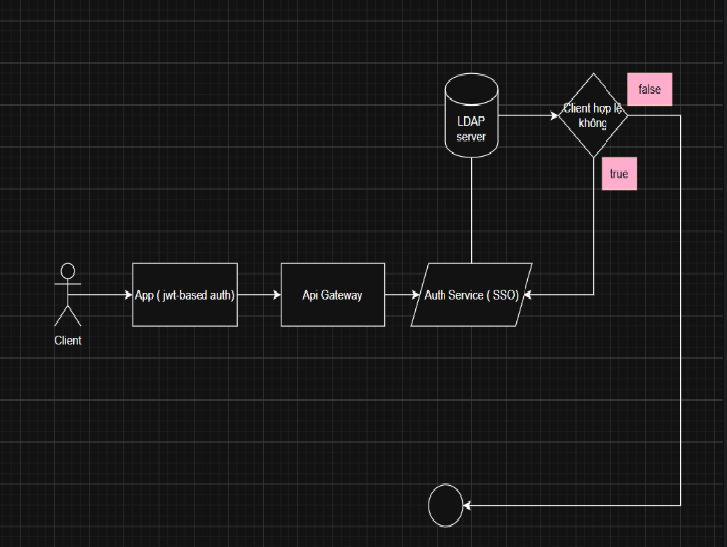
\includegraphics[width=0.95\linewidth]{img/architecture/overall_system_operation.png}
    \caption{\textit{Mô hình Vận hành và Luồng dữ liệu Tổng thể Hệ thống MyHCMUT}}
    \label{fig:sys_op}
\end{figure}

\begin{enumerate}
    \item \textbf{Tương tác Người dùng:} Cán bộ thực hiện thao tác trên màn hình điện thoại (điền form nghỉ phép, nhấn điểm danh họp, xem nhiệm vụ).
    \item \textbf{Điều phối Trạng thái Client:} Widget gọi phương thức tương ứng trong Riverpod \texttt{AsyncNotifier}.
    \item \textbf{Truy xuất Dữ liệu \& Gửi Request:} Notifier gọi Repository $\rightarrow$ Dio Client sử dụng \texttt{MultiDomainAuthInterceptor} tự động gắn Bearer Token và gửi request HTTPS tới Backend đích.
    \item \textbf{Xác thực \& Xử lý tại Backend:} Middleware giải mã Token bằng Shared Secret, Controller chuyển dữ liệu cho Service thực thi quy tắc nghiệp vụ trong Transaction bọc kín, lấy khóa \texttt{pg\_advisory\_xact\_lock}, kiểm tra trùng lịch và ghi nhận dữ liệu vào PostgreSQL.
    \item \textbf{Xử lý Sự kiện Bất đồng bộ Post-Commit:} Sau khi Transaction commit thành công, Backend bắn Event vào Kafka Topic $\rightarrow$ Consumer tiêu thụ và đẩy Push Notification qua Firebase FCM HTTP v1 tới điện thoại người liên quan.
    \item \textbf{Phản hồi \& Render Giao diện:} Backend trả về HTTP 200 kèm JSON $\rightarrow$ Client deserialize sang Freezed DTO $\rightarrow$ Cập nhật State trong Riverpod $\rightarrow$ Giao diện tự động cập nhật dữ liệu mới tức thì.
\end{enumerate}
